% \documentclass[9pt]{beamer}
\documentclass[aspectratio=169,xcolor=dvipsnames,9pt]{beamer}
\usepackage{listings}
\newcommand{\pc}[1]{\lstinline{#1}}
%%%%%%%%%%%%%%%%%%%%%%%%

\usepackage[square,numbers]{natbib}
\usecolortheme{Imperial}
\usetheme{SimplePlus}
\usepackage{appendixnumberbeamer}


\usepackage{amsfonts, amsmath, amsthm, amssymb}
\usepackage{bbm}
\usepackage{bm}
\usepackage{mathtools}


\newcommand*{\QEDA}{\hfill\ensuremath{\blacksquare}}%
\newcommand*{\QEDB}{\hfill\ensuremath{\square}}%

\setbeamertemplate{itemize items}[circle]
\setbeamertemplate{enumerate items}[default]
\setbeamerfont{title}{size=\LARGE}

\title{\textbf{Data Visualization from a\\Category Theory Perspective}}
\date{}

\begin{document}

\maketitle

\begin{frame}{Table of contents}
	\setbeamertemplate{section in toc}[sections numbered]
	\setbeamertemplate{subsection in toc}[subsections numbered]
	\setbeamerfont{subsection in toc}{size=\small}
	\tableofcontents[sectionstyle=show, subsectionstyle=show]
\end{frame}

\AtBeginSection{}
\section[Introduction]{Introduction}
\subsection[Motivation]{Motivation}
\begin{frame}[fragile]{Motivation}

	This thesis began by trying to reproduce the following plot
	within the Julia programming language.

	\begin{figure}[H]
		\begin{center}
			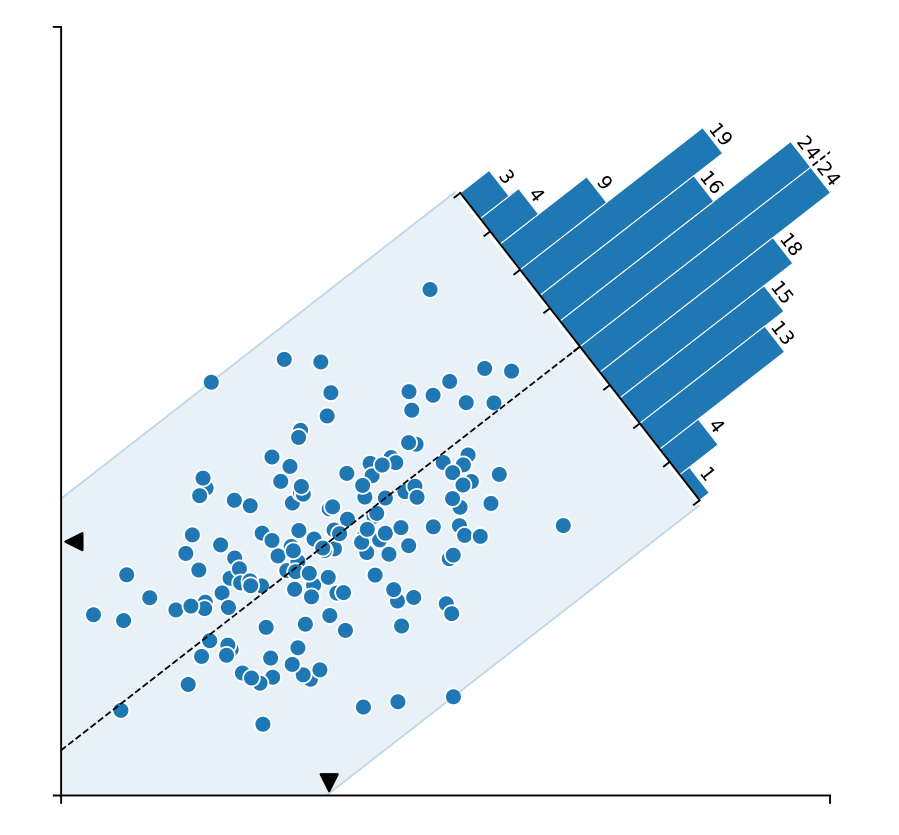
\includegraphics[width=0.35\textwidth]{./figures/rotated-histogram.png}
		\end{center}
		\caption{Rotated histogram aligned with second main PCA axis. Figure from \citet{rougier2021scientific}.}
		\label{fig:rotated-histogram}
	\end{figure}

\end{frame}

\begin{frame}[fragile]{Introduction}

	Develope a new data visualizaiton package.
	\begin{figure}
		\begin{center}
			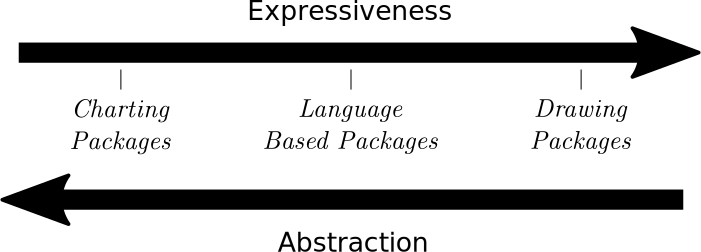
\includegraphics[width=0.85\textwidth]{./figures/expressiveness}
		\end{center}
		\caption{Expressiveness per data visualizaiton package type.}
		\label{fig:expressiveness}
	\end{figure}

\end{frame}

\begin{frame}[fragile]{Introduction}

	Scatter plot and Line plot are programmatically different.
	\begin{figure}
		\begin{center}
			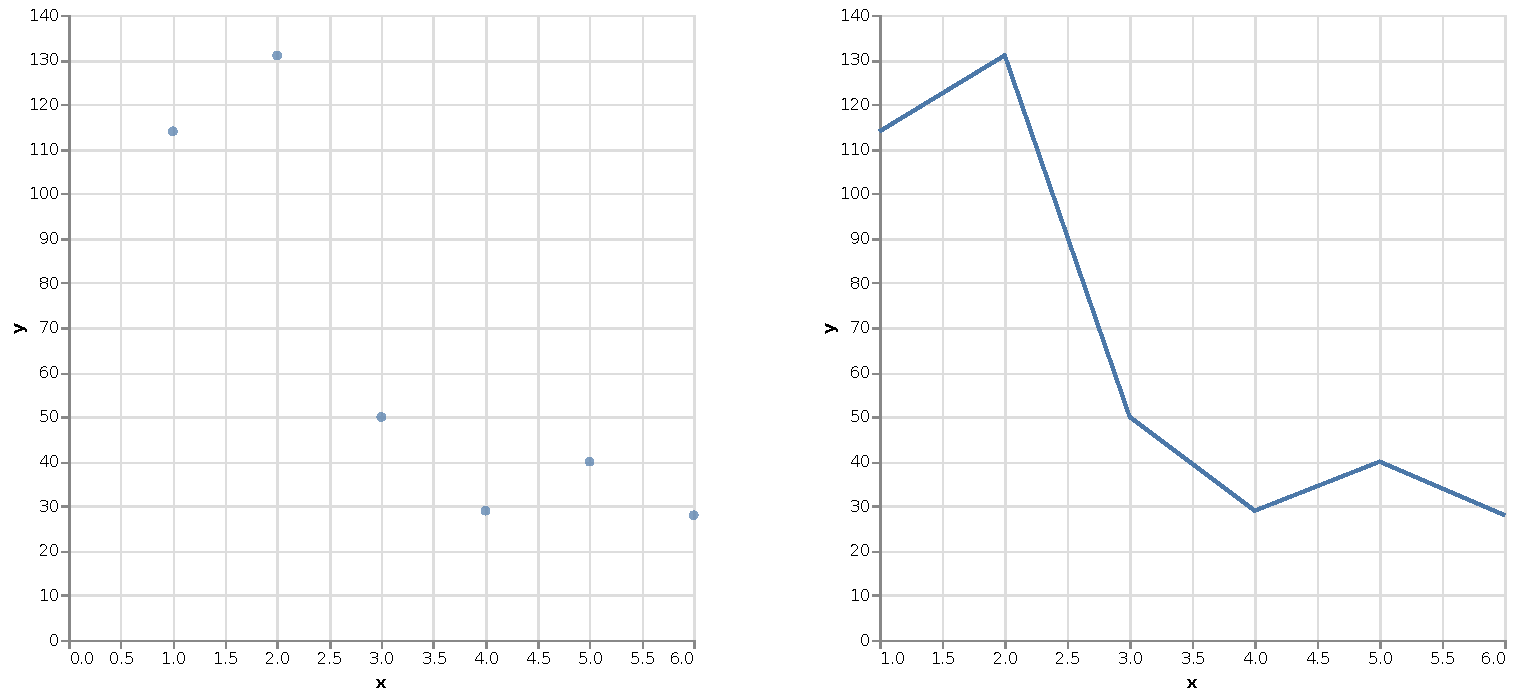
\includegraphics[width=0.85\textwidth]{./figures/scatterplot lineplot.pdf}
		\end{center}
		\caption{Expressiveness per data visualizaiton package type.}
		\label{fig:expressiveness}
	\end{figure}

\end{frame}

\begin{frame}[fragile]{Introduction}

	Surprisingly, as pointed out by \citet{chen2007handbook},
	although graphics are extensively used in
	many fields, there is still not a lot of substantive theory on the subject
	from the perspective of data visualization.
	\vspace{5mm}

	From our literature review, we were able to identify three
	seminal works that contributed to formalize the process of encoding
	data in a geometrical description:
	\begin{itemize}
		\item  Semiology of Graphics \citep{bertin1983semiology};
		\item  A Presentation Tool \citep{mackinlay1986automating};
		\item  Grammar of Graphics \citep{wilkinson2012grammar}.
	\end{itemize}

\end{frame}


\subsection[Objective]{Objective and Challenges}
\begin{frame}[fragile]{Objective and Challenges}

	\textbf{Main Objective:} Develop a new
	formalization framework for data visualization. The purpose of this framework is
	to guide the development of a general purpose data visualization library by providing sound abstraction without
	compromising expressiveness.
	\vspace{3mm}

	\textbf{Challenges}
	\vspace{2mm}

	\textit{Expressiveness}:
	\begin{itemize}
		\item Composite visualizations;
		\item Customized marks.
	\end{itemize}

	\textit{Abstraction}:
	\begin{itemize}
		\item Mathematical rigour;
		\item Visualizations constructed with an intuitive logic.
	\end{itemize}

\end{frame}

\begin{frame}[fragile]{Challenges}

	\begin{figure}[H]
		\begin{center}
			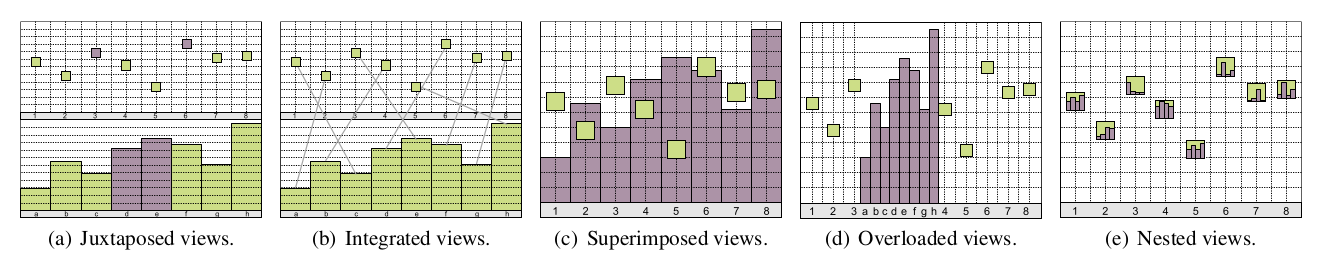
\includegraphics[width=1.\textwidth]{./figures/vizcomp.png}
		\end{center}
		\caption{Example of composing a \textit{scatter plot} and \textit{bar chart}. Taken from \citet{javed2012exploring}.}
		\label{fig:vizcomp}
	\end{figure}

\end{frame}

\begin{frame}[fragile]{Challenges}

	Example of visualization that uses customized marks.
	\begin{figure}[H]
		\begin{center}
			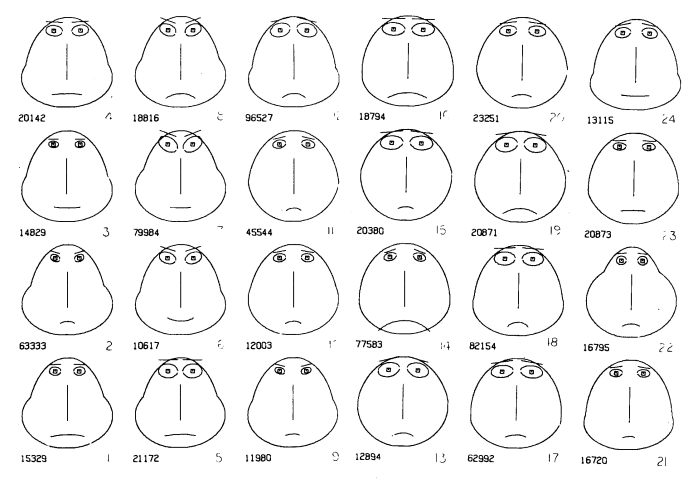
\includegraphics[width=0.55\textwidth]{./figures/chernoff_face.png}
		\end{center}
		\caption{Example of Chernoff faces from \citet{chernoff1973use}.}
		\label{fig:chernofffaces}
	\end{figure}

\end{frame}

\section[Category Theory]{Category Theory}
\subsection{Why Category Theory?}
\begin{frame}[fragile]{Why Category Theory?}
	\textbf{Category Theory} is a branch of mathematics that
	studies general abstract structures through their relationships.
	\vspace{3mm}

	\textbf{Origin: }Samuel Eilenberg e Saunders Mac Lane - 1940
	\vspace{3mm}

	As pointed by \citet{fong2019invitation}, Category Theory is unmatched
	in its ability to organize and relate abstractions. We believe that
	it may serve as a robust framework for bridging mathematics, computer science and data visualization.

	\vspace{3mm}
	\begin{figure}[H]
		\begin{center}
			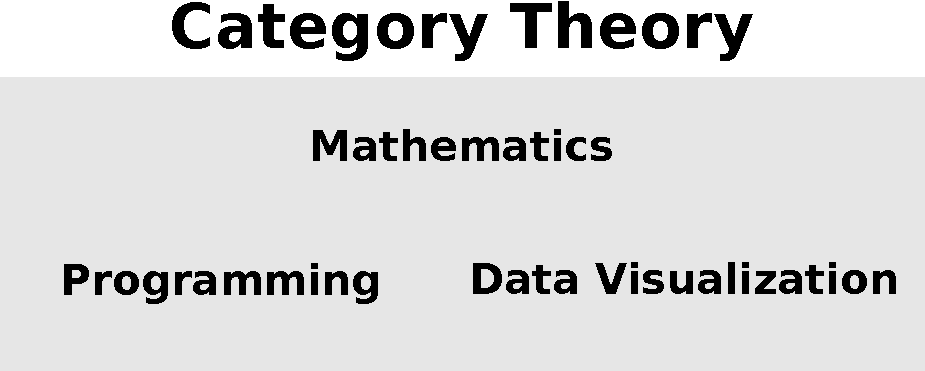
\includegraphics[width=0.40\textwidth]{./figures/category-triad.pdf}
		\end{center}
	\end{figure}
\end{frame}

\subsection[Category Theory Brief Introduction]{Category Theory Brief Introduction}
\begin{frame}[fragile]{Category Theory Brief Introduction}
	Category Theory is a branch of mathematics that
	studies general abstract structures through their relationships.

	\begin{definition}[Category]
		A category $\mathcal C = \langle \text{Ob}_{\mathcal C}, \text{Mor}_{\mathcal C} \rangle$ consists
		of a class of objects $\text{Ob}_\mathcal C$ and a class of morphisms
		$\text{Mor}_\mathcal C$. A morphism $f \in \text{Mor}_\mathcal C(A,B)$ has a domain $A \in \text{Ob}_\mathcal C$
		and a codomain $B \in \text{Ob}_\mathcal C$. Every object has an identity morphism.
		Every morphism can be composed, and this composition is associative.
	\end{definition}
\end{frame}

\begin{frame}[fragile]{Category Theory Brief Introduction}
	The category $\bm 1$ consists of $\text{Ob}_{\bm 1} := \{A\}$ and $\text{Mor}_{\bm 1} = \{id_A\}$.
	The diagram for such category is shown below.
	\begin{figure}[H]
		\begin{center}
			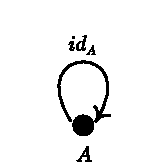
\includegraphics[width=0.15\textwidth]{./figures/1Cat}
		\end{center}
		\caption{Category $\bm 1$.}
		\label{fig:1Cat}
	\end{figure}
	The category $\bm 2$ consists of $\text{Ob}_{\bm 2} := \{A, B\}$ and $\text{Mor}_{\bm 1} = \{id_A, id_B, f\}$,
	where $f:A \to B$.
	The diagram for such category is shown below.
	\begin{figure}[H]
		\begin{center}
			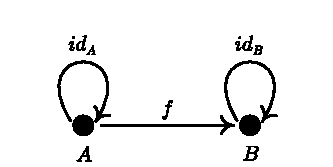
\includegraphics[width=0.30\textwidth]{./figures/2Cat}
		\end{center}
		\caption{Category $\bm 2$.}
		\label{fig:2Cat}
	\end{figure}
\end{frame}

\begin{frame}[fragile]{Category Theory Brief Introduction}
	The category $\bm 3$ has three morphisms besides the identities. The morphisms are
	$f$, $g$ and their composition $g \circ f$. The figure below
	illustrates the category with all its morphisms.
	\bigskip
	\begin{figure}[H]
		\begin{center}
			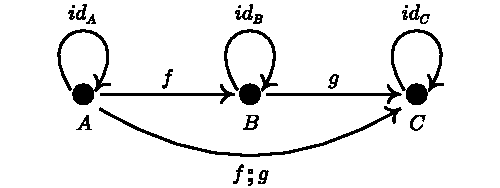
\includegraphics[width=0.50\textwidth]{./figures/3CatComplete}
		\end{center}
		\caption{Category $\bm 3$ showing all morphisms.}
		\label{fig:3Catcomplete}
	\end{figure}
\end{frame}

\begin{frame}[fragile]{Category Theory Brief Introduction}
	Here are some more interesting
	categories:
	\begin{enumerate}[1.]
		\item $\mathbf{Set}$ which is the category of sets, where the objects are sets and the morphisms are functions between sets.
		\item $\mathbf{Top}$ is the category where topological spaces are the objects and continuous functions are the morphisms.
		\item $\mathbf{Vec}_\mathbb F$ is the category where vector spaces over field $\mathbb F$ are the objects,
		      and linear transformations are the morphisms.
		\item $\mathbf{Gr}$ is the category of directed graphs, where $\text{Ob}_{\mathbf{Gr}} := \{\text{Vertex}, \text{Arrow}\}$,
		      and the morphisms are
		      \begin{displaymath}
			      \text{Mor}_{\mathbf{Gr}} := \{
			      src,
			      tgt,
			      id_{\text{Vertex}},
			      id_{\text{Arrow}}
			      \}
		      \end{displaymath}
		      where $src:\text{Arrow} \to \text{Vertex}$ returns the source vertex for each arrow and
		      $tgt:\text{Arrow} \to \text{Vertex}$ returns the target vertex.
	\end{enumerate}
\end{frame}

\begin{frame}[fragile]{Category Theory Brief Introduction}
	Objects defined in terms of existence and
	uniqueness of morphisms are known as \textbf{universal constructions}.
	\begin{definition}[Zero, Initial and Terminal]
		Let $\mathcal C$ be a category.
		\begin{enumerate}[1.]
			\item An object $I \in \text{Ob}_\mathcal C$ is \textit{initial} if for every $A \in \text{Ob}_\mathcal C$,
			      there is exactly one morphism from $I$ to $A$. Thus, from $I$ to $I$ there is only the identity.
			\item An object $T \in \text{Ob}_\mathcal C$ is \textit{terminal} if for every $A \in \text{Ob}_\mathcal C$,
			      there is exactly one morphism from $A$ to $T$. Thus, from $I$ to $I$ there is only the identity.
			\item An object is \textit{zero} if it is both terminal and initial.
		\end{enumerate}
	\end{definition}
\end{frame}

\begin{frame}[fragile]{Category Theory Brief Introduction}
	\begin{definition}[Functor]
		Let $\mathcal C$ and $\mathcal D$ be two categories. A functor $F: \mathcal C \to \mathcal D$ is
		a pair of mappings with the following properties:
		\begin{figure}[H]
			\begin{center}
				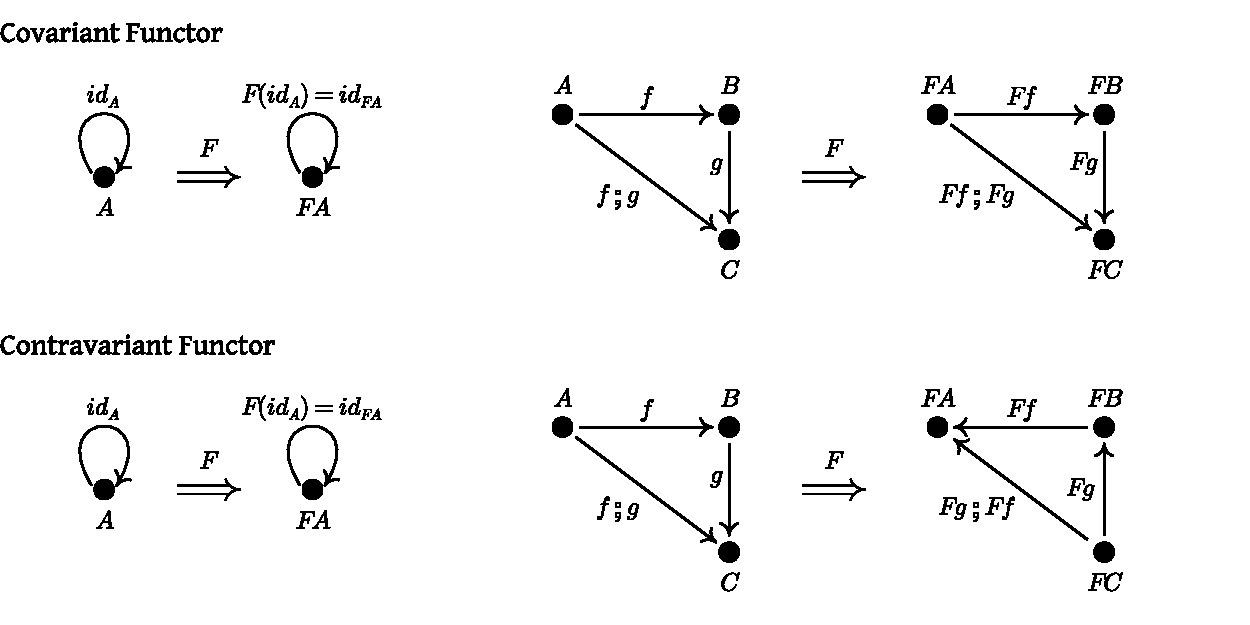
\includegraphics[width=0.8\textwidth]{./figures/Functor.pdf}
			\end{center}
			\caption{Diagrams showcasing the properties of functors.}
			\label{fig:Functor}
		\end{figure}
	\end{definition}

\end{frame}

\begin{frame}[fragile]{Category Theory Brief Introduction}
	\begin{definition}[Natural Transformations]
		Let $\mathcal C$ and $\mathcal D$ be categories, and let $F,G:\mathcal C \to \mathcal D$ be functors.
		A natural transformation $\alpha: F \to G$ is such that the following diagram commutes:
		\begin{figure}[H]
			\begin{center}
				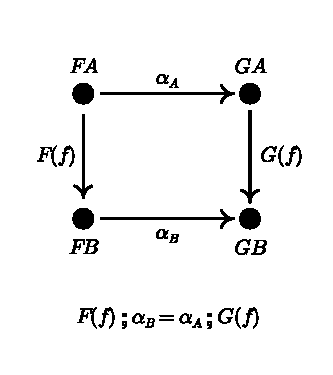
\includegraphics[width=0.35\textwidth]{./figures/NaturalTransformation.pdf}
			\end{center}
			\caption{Commutative diagram of a natural transformation highlighting the commutative property of the definition.}
			\label{fig:NaturalTransformation}
		\end{figure}
	\end{definition}
\end{frame}

\begin{frame}[fragile]{Category Theory Brief Introduction}
	\textbf{Monoids} and \textbf{Monads} are two ubiquitous constructions both in Category Theory and
	Functional Programming. These two concepts will be used when talking about
	data visualization. Therefore, it is required of us to introduce these constructions.

	Let's start with the definition of a monoid in the context of Set Theory.

	\begin{definition}[Monoid - Set Theory]
		A monoid is a triple $(M, \otimes, e_M)$ where $M$ is a set, $\otimes:M\times M \to M$ is a binary operation
		and $e_M$ the neutral element, such that:
		\begin{enumerate}
			\item $a \otimes (b \otimes c) = (a \otimes b) \otimes c$
			\item $a \otimes e_M = e_M \otimes a = a$.
		\end{enumerate}
		\label{def:monoid}
	\end{definition}

	An example of a monoid is $(\mathbb N \cup \{0\}, +, 0)$.
	It is easy to check that the summation operator satisfies the
	associativity neutrality properties.
\end{frame}

\begin{frame}[fragile]{Category Theory Brief Introduction}
	\begin{definition}[Monoid in the  category $\mathbf{Set}$]
		A monoid in $\mathbf{Set}$ is a triple $(M, \mu, \eta)$, where $M \in \text{Ob}_\mathbf{Set}$,
		$\mu:M \times M \to M$ and $\eta: 1 \to M$ are two morphisms in $\mathbf{Set}$ satisfying the
		commutative diagrams below. Note that $1$ is the terminal object in $\mathbf{Set}$, i.e.
		the singleton set (which is unique up to an isomorphism).

		\begin{figure}[H]
			\begin{center}
				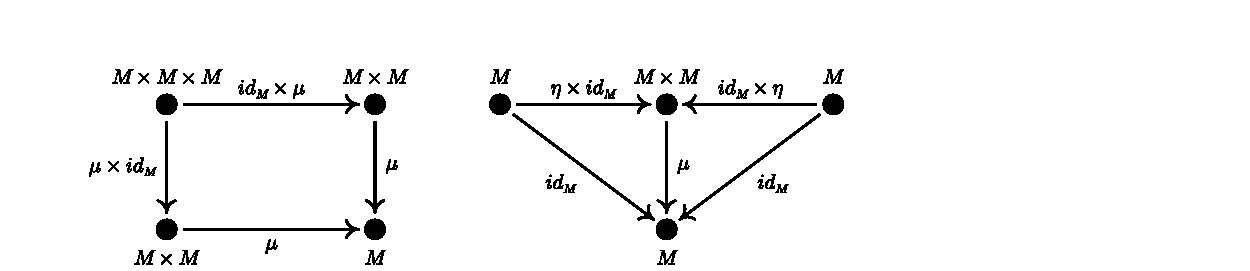
\includegraphics[width=1.3\textwidth]{./figures/MonoidalCategory.pdf}
			\end{center}
			\caption{Commutative diagram for monoid.}
			\label{fig:monoid-diagram}
		\end{figure}
		\label{def:monoid-cat}
	\end{definition}
\end{frame}

\begin{frame}[fragile]{Category Theory Brief Introduction}
	\begin{definition}[Monad]
		A monad is a monoid in $\mathbf{End}_\mathcal C$, which is the triple $(T, \mu, \eta)$,
		where $T:\mathcal C \to \mathcal C$ is a functor,
		$\mu:T \circ T \to T$ and $\eta: 1 \to T$ are natural transformations in $\mathbf{End}_\mathcal C$ satisfying the
		commutative diagrams \ref{fig:monad}. Note that $1$ is the identity functor in $\mathcal{C}$.
		\begin{figure}[H]
			\begin{center}
				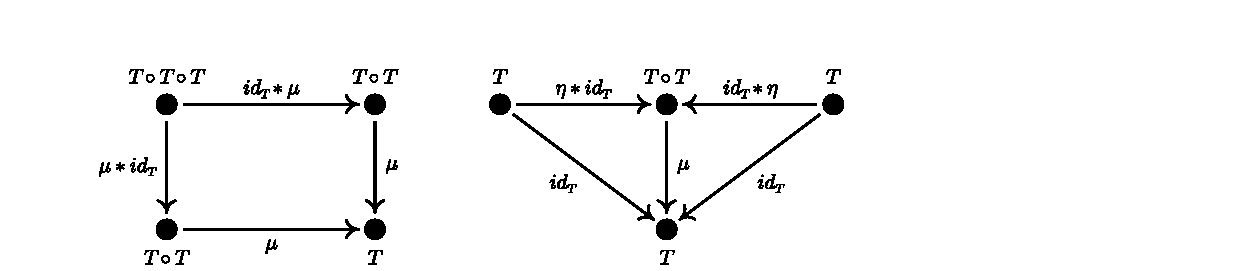
\includegraphics[width=1.3\textwidth]{./figures/Monad.pdf}
			\end{center}
			\caption{Commutative diagram for monad.}
			\label{fig:monad}
		\end{figure}
	\end{definition}
\end{frame}

\begin{frame}[fragile]{Applied Category Theory}
	\textbf{Programming}
	\vspace{3mm}

	One of the most common applications is in Programming,
	where Category Theory can presents a strong connection with the Functional Programming paradigm.

	\begin{definition}[Category $\mathbf{Prog}(L)$]
		Category $\mathbf{Prog}(L)$ is a subcategory of $\mathbf{Set}$ where programming
		types are the objects and correspond to a set. The morphisms are pure
		referentially transparent and terminating functions, which correspond to
		functions in $\mathbf{Set}$. If two functions in $L$ are denotationally the same,
		i.e. for every \pc{x::T} we have \pc{f(x) = g(x)}, then they correspond
		to the same function in $\mathbf{Prog}(L)$.
	\end{definition}
\end{frame}

\section[An Application in Data Visualization - Diagrams]{An Application in Data Visualization - Diagrams}
\subsection[Data Visualization Pipeline]{Data Visualization Pipeline}
\begin{frame}[fragile]{An Application in Data Visualization - Diagrams}

	\begin{figure}[h]
		\begin{center}
			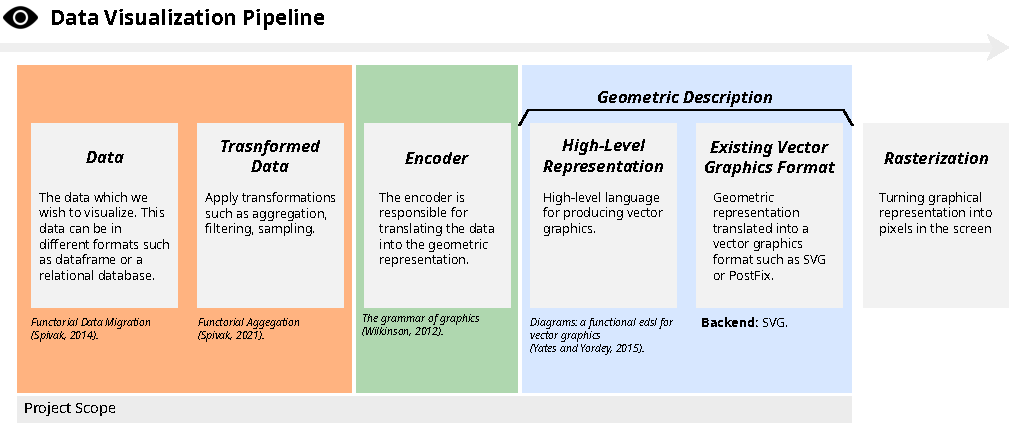
\includegraphics[width=1\textwidth]{./figures/datavizscope.pdf}
		\end{center}
		\caption{Visualization pipeline.}
		\label{fig:datavizpipeline}
	\end{figure}
\end{frame}

\subsection[Diagrams]{Diagrams as Monoids}
\begin{frame}[fragile]{Category Theory for Diagrams}
	\textbf{Diagrams as Monoids}
	\vspace{3mm}

	\citet{yorgey2012monoids} proposed a Domain-Specific Language which models
	the process of generic diagram creation.
	The paper explains some of the ideas that went behind the development
	of the framework \textit{Diagrams} \citep{yates2015diagrams},
	which is a Haskell library for drawing diagrams.
	\begin{figure}[H]
		\begin{center}
			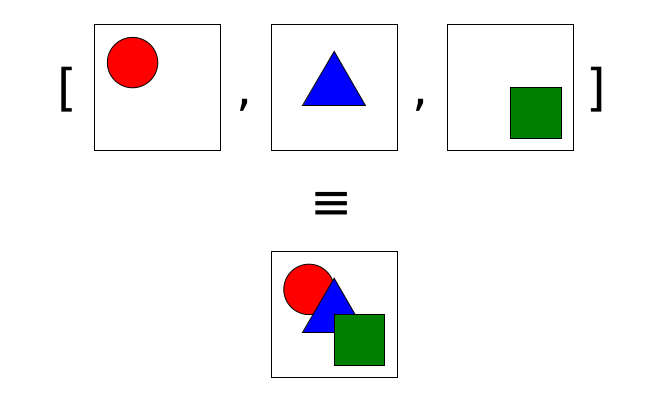
\includegraphics[width=0.40\textwidth]{./figures/diagrams.png}
		\end{center}
		\caption{Example of how a diagram works. Image from \citet{yorgey2012monoids}.}
		\label{fig:diagrams}
	\end{figure}
\end{frame}

\begin{frame}[allowframebreaks]{References}
	% \nocite{*}
	\renewcommand{\section}[2]{}%
	\tiny{\bibliography{../ref}}
	\bibliographystyle{plainnat}
\end{frame}

\end{document}
